% ответы на вопросы
\newpage
\section*{Результаты работы}
\addcontentsline{toc}{section}{\tocsecindent{Результаты работы}}

\subsection*{Задание 1}
Графики зависимости от времени импульса $t$ при методе Рунге-Кнутта 4-го порядка точности.
\begin{figure}[h]
	\caption{График $I(t)$}
	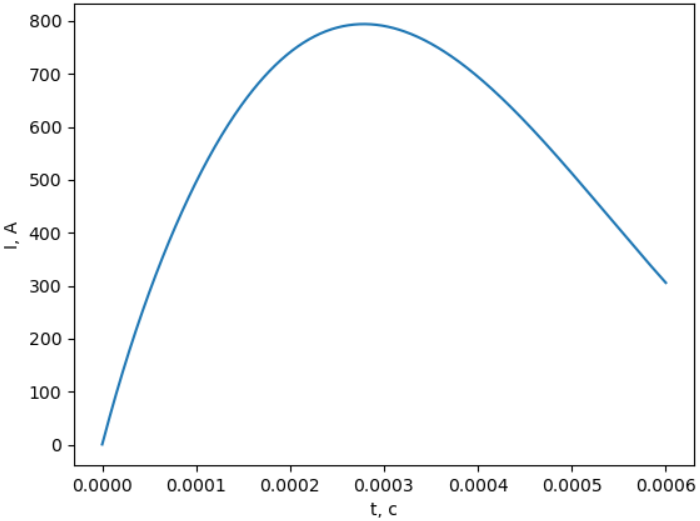
\includegraphics[scale=0.45]{img/1.png}
\end{figure}
\begin{figure}[h]
	\caption{График $U(t)$}
	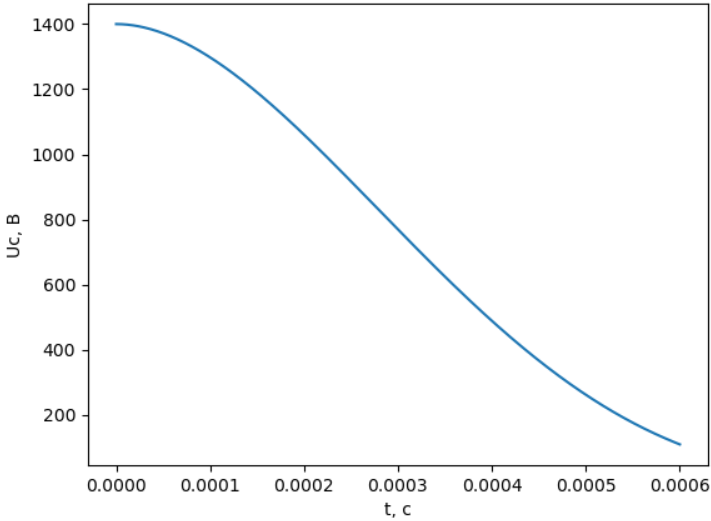
\includegraphics[scale=0.45]{img/2.png}
\end{figure}
\begin{figure}[h]
	
	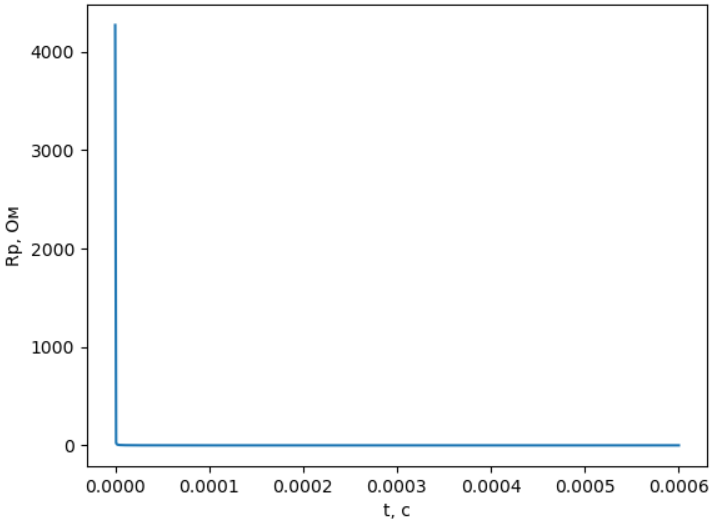
\includegraphics[scale=0.45]{img/3.png}
	\caption{График $R_p(t)$}
\end{figure}
\newpage
\begin{figure}[h]
	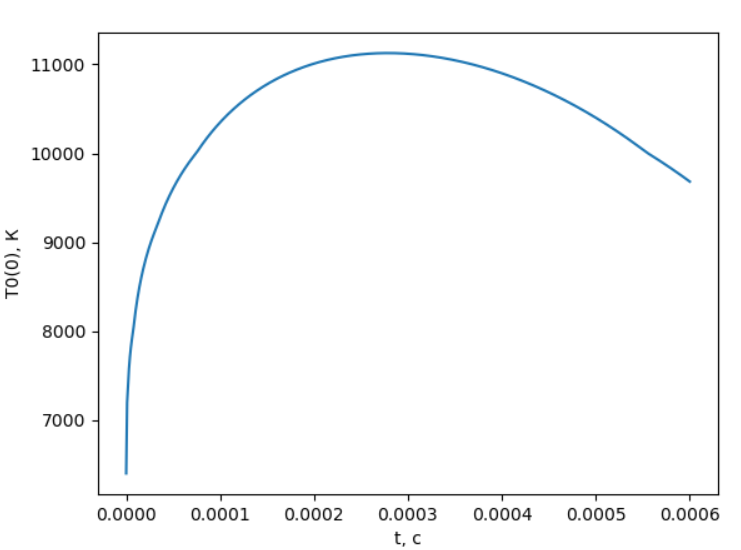
\includegraphics[scale=0.45]{img/4.png}
	\caption{График $I(t)\cdot R_p(t)$}
\end{figure}
\begin{figure}[h!]
	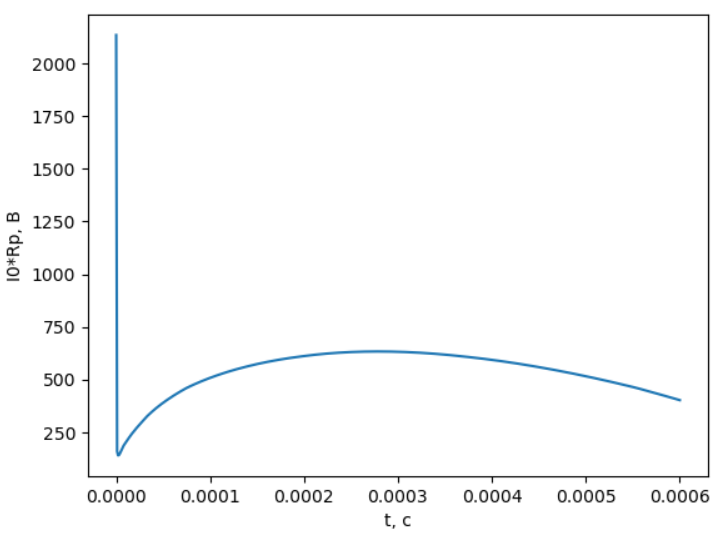
\includegraphics[scale=0.45]{img/5.png}
	\caption{График $T_0(t)$}
\end{figure}
Теперь построим для метода Рунге-Кнутта 2-го порядка точности график зависимости $T_0$ от $t$:
\begin{figure}[h!]
	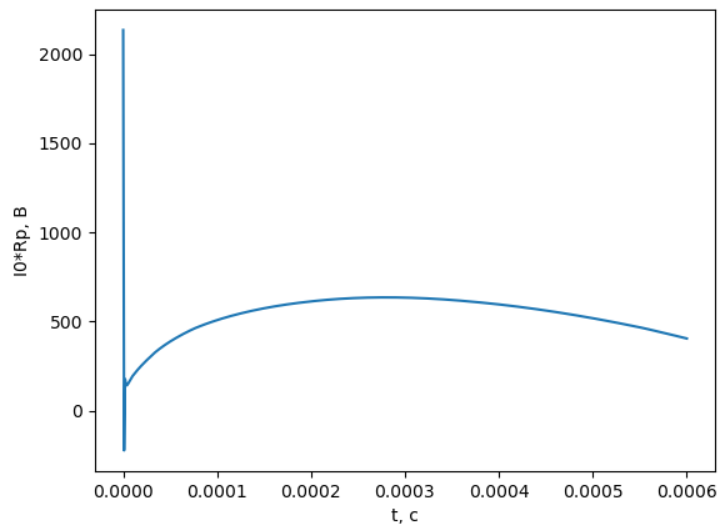
\includegraphics[scale=0.45]{img/6.png}
	\caption{График $T_0(t)$}
\end{figure}
\newpage
\subsection*{Задание 2}
График зависимости $I(t)$ при $R_k+R_p=0$.
\begin{figure}[h!]
	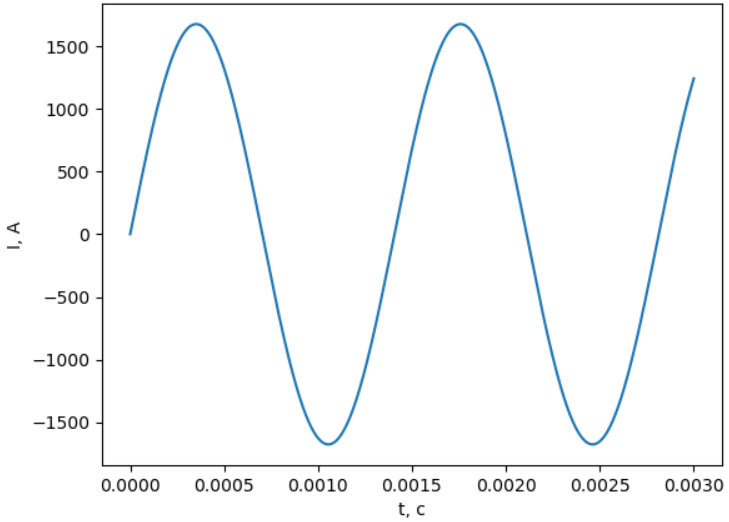
\includegraphics[scale=0.6]{img/7.png}
	\caption{График $I(t)$}
\end{figure}
\newline Из графика видно, что колебания действительно стали незатухающими.
\subsection*{Задание 3}
График зависимости $I(t)$ при $R_k = 200$ Ом в интервале значений $t$ $0-20$ мкс.
\begin{figure}[h!]
	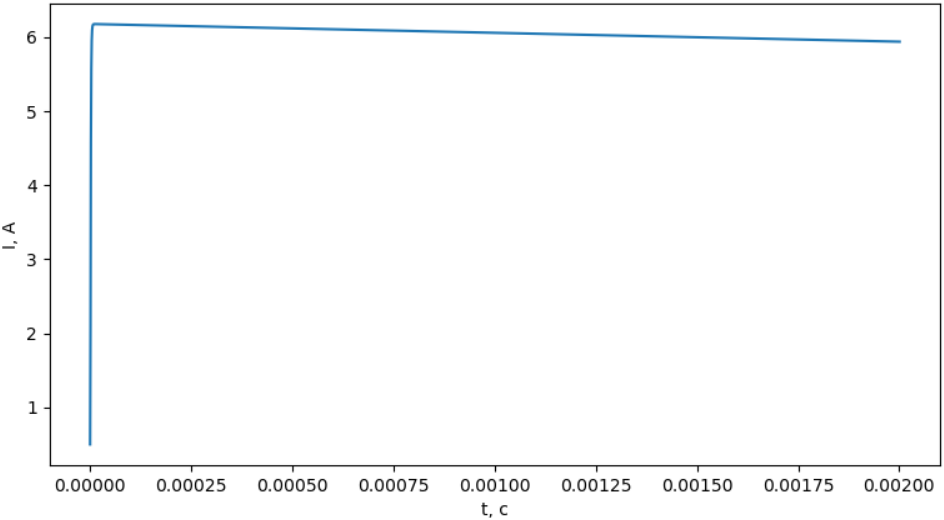
\includegraphics[scale=0.6]{img/8.png}
	\caption{График $I(t)$}
\end{figure}

\section*{Ответы на вопросы}
\addcontentsline{toc}{section}{\tocsecindent{Ответы на вопросы}}

\textbf{1. Какие способы тестирования программы можно предложить?}\\

Первый способ: поставить довольно большое сопротивление (200-250 Ом). В таком случае следует уменьшить шаг (например, до 1e-7), чтобы захватить момент резкого увеличения силы тока.

Второй способ: сделать $R_k$ и $R_p$ равными нулю. Тогда потерь в контуре не будет и на графике отобразится идеальная бесконечная синусоида.

Третий способ: сделать $R_k$ равным какому-то небольшому константному значению (например, 1 Ом). В этом случае синусоида должна быть затухающей, а задачу следует решать аналитически.\\
\textbf{2. Получите систему разностных уравнений для решения сформулированной задачи неявным методом трапеций. Опишите алгоритм реализации полученных уравнений.}\\
Используя систему (1):
\begin{equation}
\begin{cases}
\frac{dI}{dT} = \frac{U - (R_k + R_p(I))I}{L_k} \equiv f(I, U_c)\\
\frac{dU}{dt} = -\frac{I}{C_k} 	\equiv g(I)\\
\end{cases}
\end{equation}
Запишем выражения для метода:
\begin{equation}
\begin{cases}
I_{n+1}=I_n + \Delta t \frac{f(I_n,U_{cn})+f(I_{n+1},U_{cn+1})}{2}\\
U_{cn+1}= U_{cn}+\Delta t \frac{g(I_n) + g(I_{n+1})}{2}\\
\end{cases}
\end{equation}
Подставим в (7) выражения f и g из (6):
\begin{equation}
\begin{cases}
	I_{n+1}=I_n + \Delta t \frac{U_{cn}-(R_k +R_p(I_n))I_n+U_{cn+1}-(R_k+R_p(I_{n+1}))I_{n+1})}{2L_k}\\
	U_{cn+1}= U_{cn}-\Delta t \frac{I_n + I_{n+1}}{2C_k}\\
\end{cases}
\end{equation}
Подставим $U_{cn+1}$ в верхнее уравнение и решим его относительно $I_{n+1}$:
\begin{equation}
I_{n+1}=\frac{-2C_kR_p(I_n)I_n\Delta t + 4C_kL_kI_n-2C_kI_nR_k\Delta t+4C_kU_{cn}\Delta t - I_n\Delta t^2}{4C_kL_k + 2C_kR_k\Delta t + 2 C_kR_p(I_{n+1})\Delta t+ \Delta t^2}
\end{equation}
Поскольку в правой части фигурирует $R_p(I_{n+1})$, следует решить это уравнение методом простой итерации (10).
\begin{eqnarray}
x^{(s)}=f(x^{(s-1)})
\end{eqnarray}
Полученное подставляем в (7) и находим $U_{cn+1}$ по указанной формуле:
\begin{equation}
U_{cn+1}= U_{cn}+\Delta t \frac{g(I_n) + g(I_{n+1})}{2}
\end{equation}
\textbf{3. Из каких соображений проводится выбор того или иного метода, учитывая, что чем выше порядок точности метода, тем он более сложен?}\\
Выбор зависит от степени точности метода, требуемой для конкретной задачи и от доступного количества ресурсов(объемов памяти)/времени.


